\documentclass[11pt,letterpaper]{article}
%\documentclass[11pt,a4paper]{report}

\usepackage{amssymb,amsmath,amsthm} 
\usepackage[margin=2cm]{geometry}
\usepackage{fancyhdr}
\usepackage{enumitem}
\usepackage[compact]{titlesec}
\usepackage{graphicx,ctable,booktabs,subcaption}

\usepackage{xparse,hyperref,parskip}

%\newcommand{\abs}[1]{\left|#1\right|}

\newcommand{\semester}{Spring 2022}
\newcommand{\due}{Tuesday, April 19}

\newcommand{\bigo}{\mathcal{O}}

\pagestyle{fancy}
\lhead{ }
\chead{\footnotesize Math 3338\quad  Numerical Methods\quad  \semester}
\rhead{\footnotesize \thepage}
\setlength{\parindent}{0cm}
\setlist{noitemsep}



\newtheorem{theorem}{Theorem}

\input{defs.tex}

%Defines the problem environment with arguments Points and Solution gap
\input{problem_env.tex}



\begin{document}

\begin{center}
{\huge{\bf  Numerical Methods}} \\[1.5ex]
{\bf Math 3338 -- \semester}\\[1.5ex]
{\Large{\bf Worksheet 25\ \\[2ex] Discrete Fourier Transforms}}\\
\end{center}
\vspace{2mm}


\section{Reading}

\begin{table}[!ht]
 \centering
 \begin{tabular}{lc}
   CP &  7.2, 7.3, 7.4 \\
 NMEP &  -
 \end{tabular}
\caption{Sections Covered}
\end{table}

\section{Motivation}

Most functions that you'll encounter don't have a nice closed form expression. In fact, most functions
will be given by sampling some event. For example, music. Music is typically sampled at 44.1 kHz or
44,100 sample per second. When you're listening to music you're not hearing a continuous stream of 
music you're hearing a new data point every 1/44,100 seconds. This is also common in the sciences
when you are measuring an experiment. 

Figure \ref{fig:raw_data} shows an example of a function obtained through measurement. 
\begin{figure}[!ht]
 \centering
 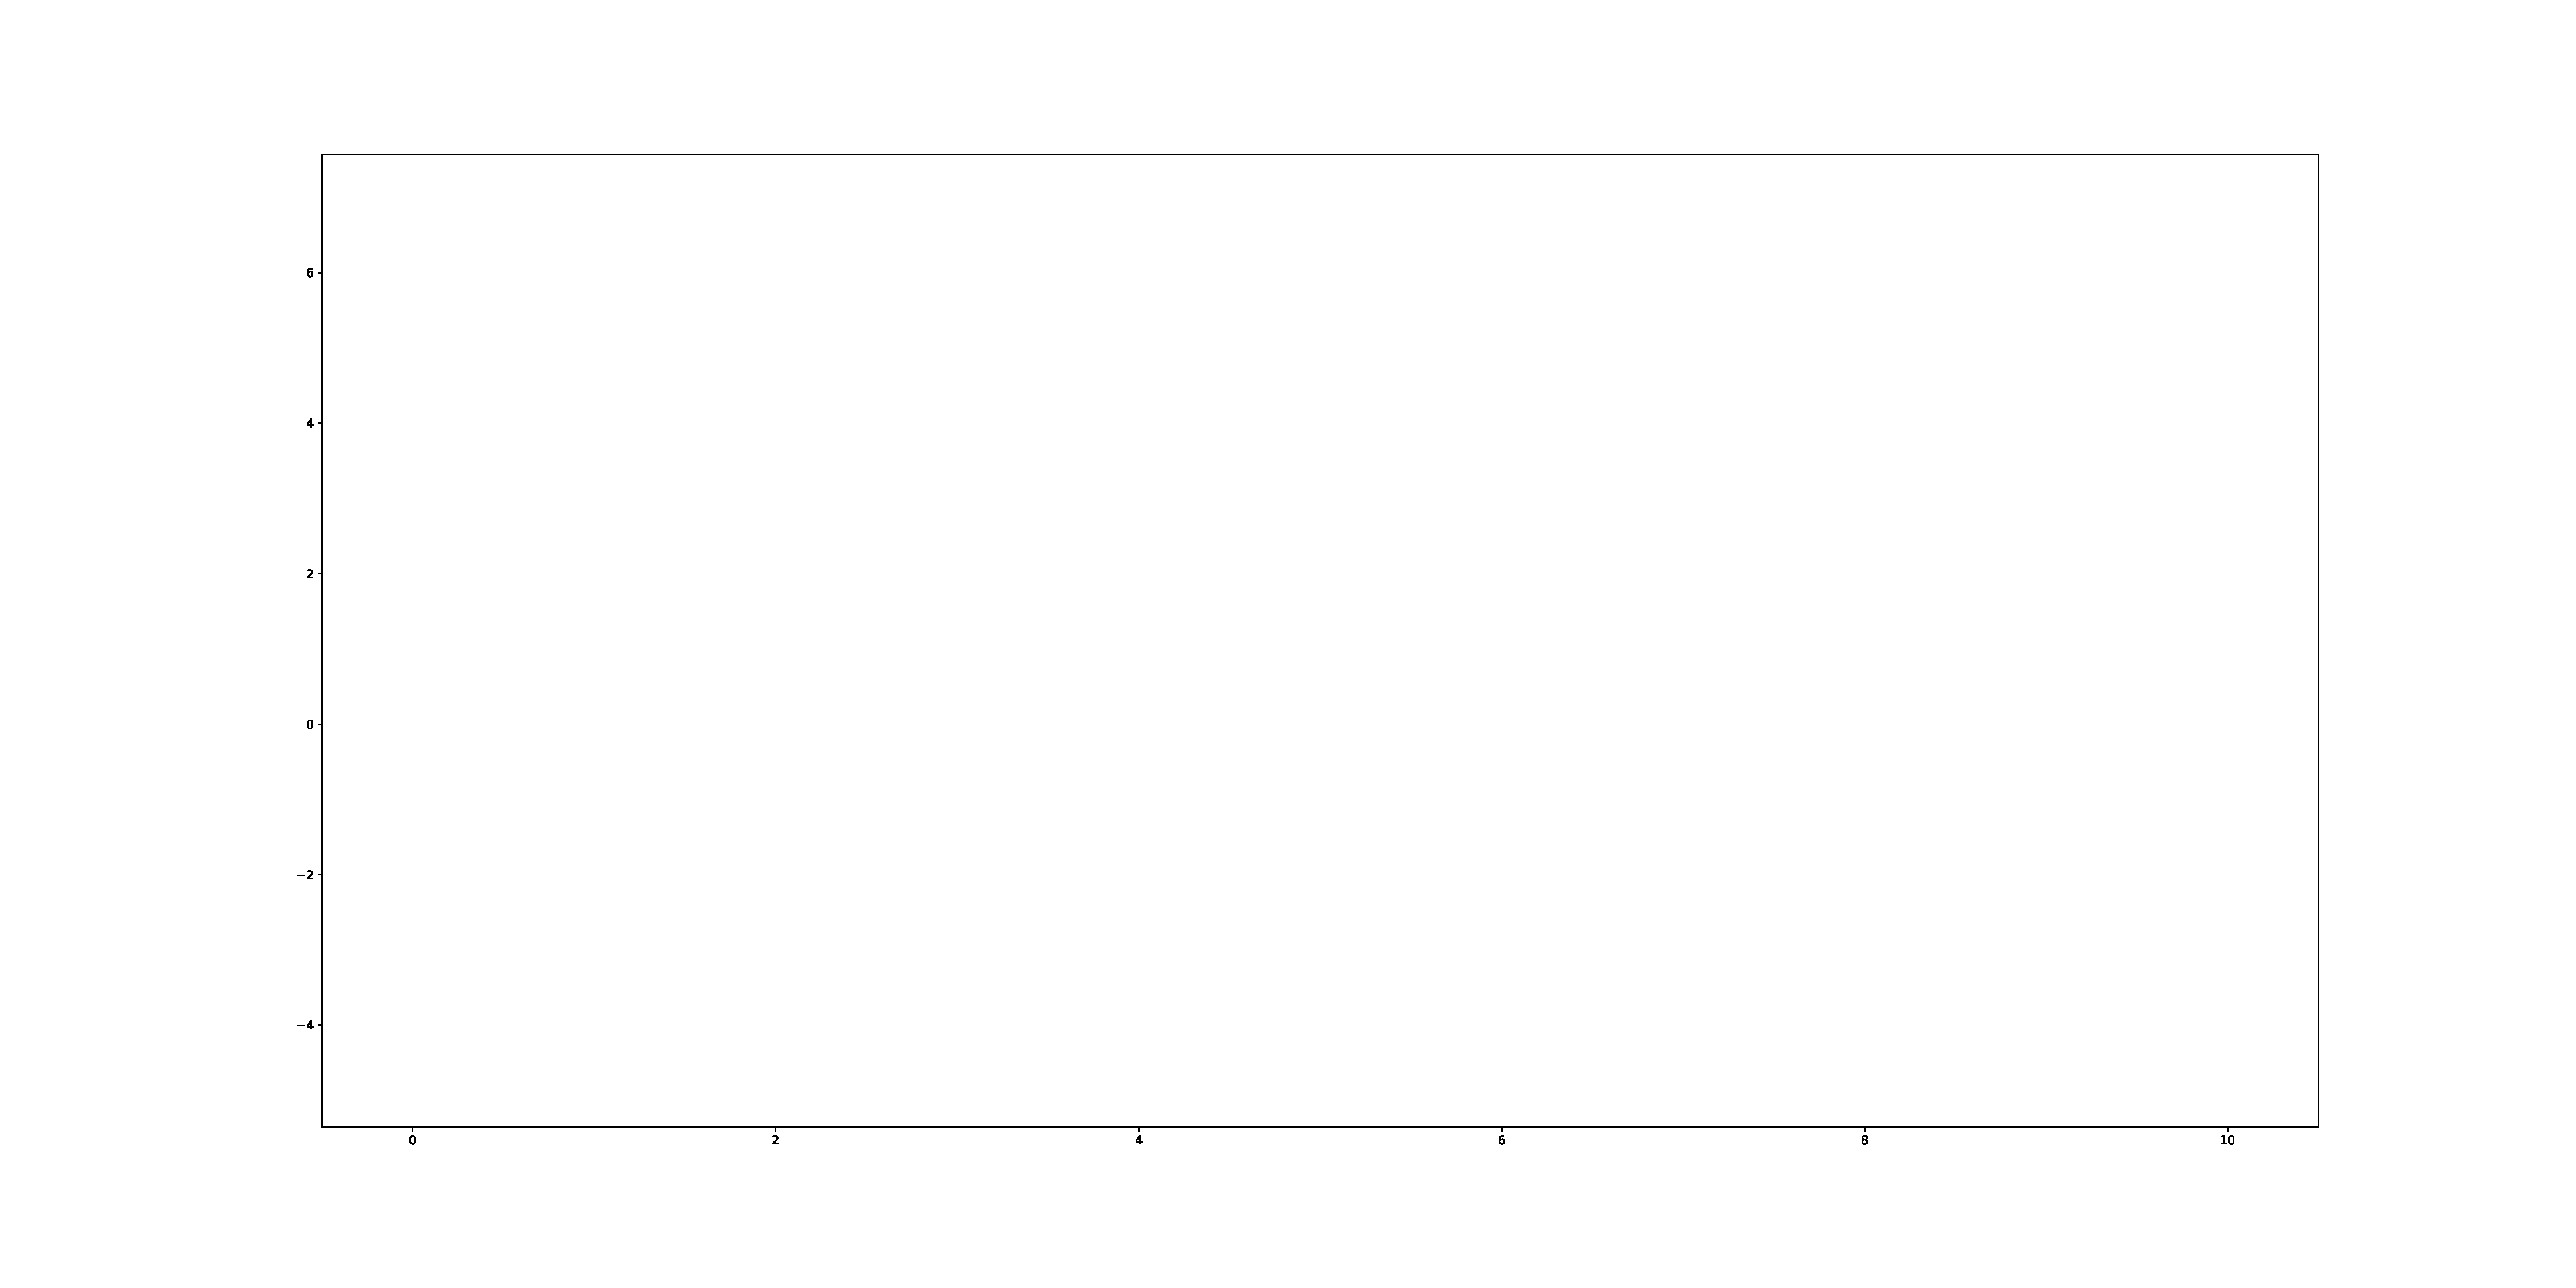
\includegraphics[width=.6\textwidth]{images/raw_data.pdf}
 \caption{The raw data}
 \label{fig:raw_data}
\end{figure}
Notice this data is very noisy, there is definitely an underlying pattern but at the moment it is
difficult to spot. This noise could be considered a consequence of a high frequency pattern in the
data. If we had a way to identify the underlying frequencies and remove the higher ones, we could
clean up this data.


Figure \ref{fig:cleaned_data} shows the above data with any frequency with an amplitude less than
$30$ filtered out. 
\begin{figure}[!ht]
 \centering
 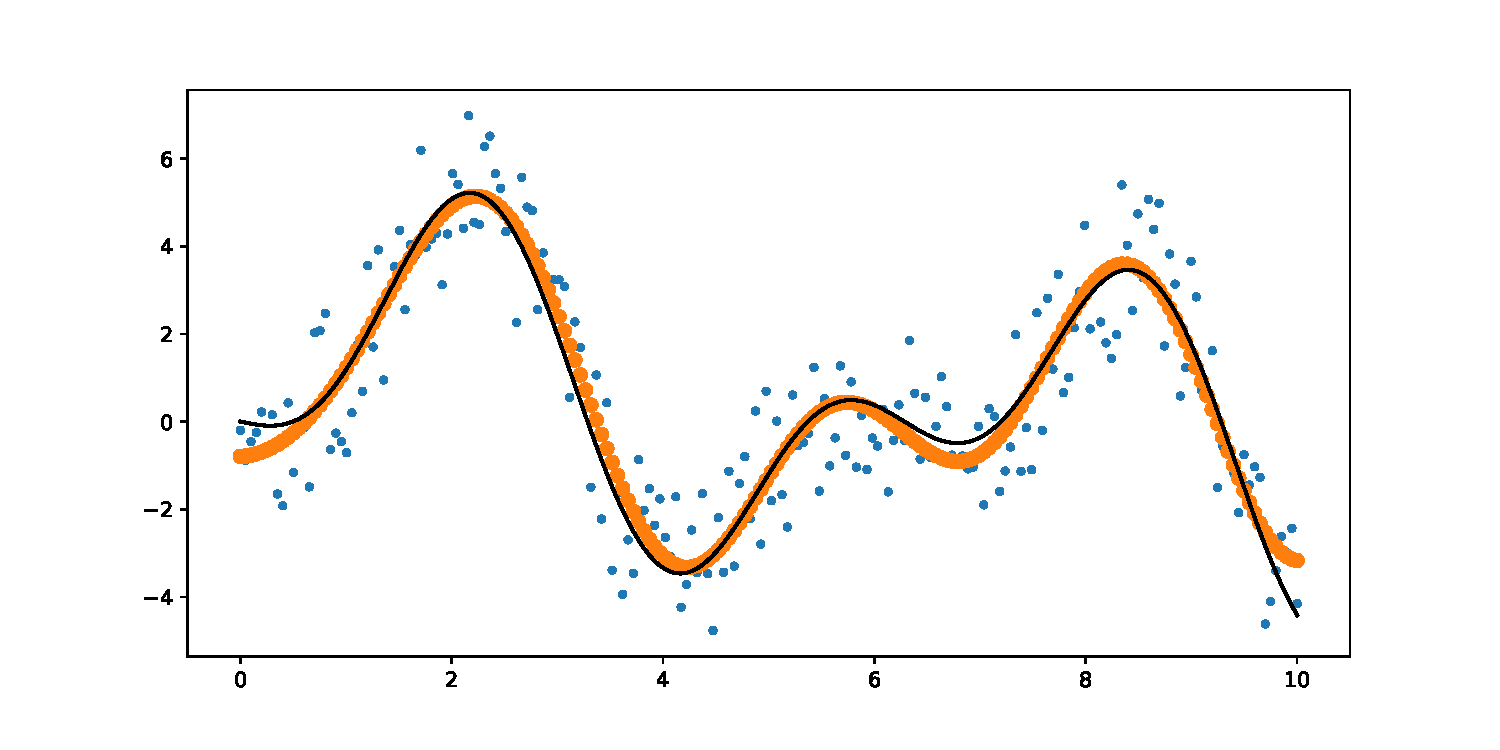
\includegraphics[width=.6\textwidth]{images/cleaned_data.pdf}
 \caption{A better fit and the exact line}
 \label{fig:cleaned_data}
\end{figure}
In other words, frequencies that weren't contributing much to the data. Notice, the orange data is
much closer to the exact black line. The orange data is constructed from 7 frequencies. There are
200 blue data points. This means we can reconstruct the 200 data points using 7 data points and 
get a ``better'' approximation of the actual curve. This is one of the key concept behind data 
compression, represent a lot of data with a little data.



\section{The Discrete Cosine Transform}

This was difficult to research. Any computer science source cared only about the implementation
with limited detail on WHY it worked. Any math source cared only for the generalizations with
very little detail on HOW it worked. I'll try to bridge the gap.

Suppose we have a sequence of points $x_n$ sampled at equally spaced points. These $x_n$ could
be the blue points in Figure \ref{fig:raw_data}. These $x_n$ are y-values, yes that
is confusing. The corresponding $x$-values turn out to not be relevant, they disappear in the 
calculations. This does rely on the $x$-values being equally spaced, if the points aren't equally 
spaced it makes the computations more complicated\footnote{The first step to solving non-uniform 
problems is a transformation to a uniform problem}. 


We want to find the frequencies $k$ and the amplitudes $X_k$. The basic idea to start with the Fourier
transformation from last time, change the integral to a sum, and do some algebra to simplify. This
is fully worked in the text. 

Suppose we have $N$ data points. The \emph{discrete Fourier transform} is given by,
\begin{equation}
\label{eqn:dct}
X_k = 2\sum_{n=0}^{N-1} x_n\cos\left(\frac{\pi k}{N}\left(n+\frac{1}{2}\right)\right)
\end{equation}
and the inverse discrete Fourier transform is given by,
\begin{equation}
\label{eqn:idct}
x_n = \frac{1}{2N}\left(X_0 + 2\sum_{k=1}^{N-1} X_k\cos\left(\frac{\pi k}{N}\left(n+\frac{1}{2}\right)\right)\right)
\end{equation}

All this is doing is transforming the points $x_n$ into points $X_k$. The real power is what these 
point represent. The $X_k$ represent amplitudes of frequencies. By setting some of these to
be zero (or deleting them) we can remove high (or low) frequency signals, or compress the data. 
That's how Figure \ref{fig:cleaned_data} was created. Any frequency with an amplitude less than
30 was killed. 






\newpage

\begin{center}
{\huge{\bf  Numerical Methods}} \\[1.5ex]
{\bf Math 3338 -- \semester}\\[1.5ex]
{\Large{\bf Homework 25 (Due: \due)}}\\
\end{center}
\vspace{2mm}

Include all graphs in your write up of the problems.



\begin{problem}
 Implement two functions \texttt{discrete\_fourier} and \texttt{inverse\_discrete\_fourier}.

\texttt{discrete\_fourier} The only input is an array $x$ that contains the $x$-values. The
output should be an array with 2 columns, the first column is the frequency and the second
is the $X_k$ values.

\texttt{inverse\_discrete\_fourier} The inputs should be a two column array (similar to the 
output of the previous) and the number of data points you want returned (this should be
the length of the $x$ vector from the previous).
\end{problem}



\begin{problem}
 On Canvas you'll find a file called ``prob2\_data.txt". This is the data from Figure 
\ref{fig:raw_data}. Take the discrete Fourier transform of this data.
\begin{enumerate}
 \item Make a plot of the amplitude vs the frequency.
 \item Filter some of the higher frequencies (or lower amplitudes). You should use array manipulation
for this. Check Worksheet 10 for a description. Do not use a list and do not use a for loop.
 \item Run the inverse Fourier transformation on the filtered array.
 \item Plot the data and the result of the inverse Fourier transform on the same axes. 
 \item Describe what you see.
\end{enumerate}
\end{problem}


\begin{problem}
\label{prob:base}
The inverse Fourier transform is just a summation of a bunch of cosines of different frequencies. 
To prove this point, you'll be plotting each individual cosine graph, the exact function, and
the sum of the cosines on the same axes. See Figure \ref{fig:base}. Your goal is to recreate 
these images. Write a function called \texttt{base\_curves} that has inputs $f$ (a function),
$x$ (a sequence of $x$-values), max\_amp (a cut-off value so you only plot certain frequencies),
and out\_name (defaults to \texttt{None}, the name of the saved graph if it's not None).

\begin{figure}[!ht]
\centering
\begin{subfigure}{.48\textwidth}
\centering
 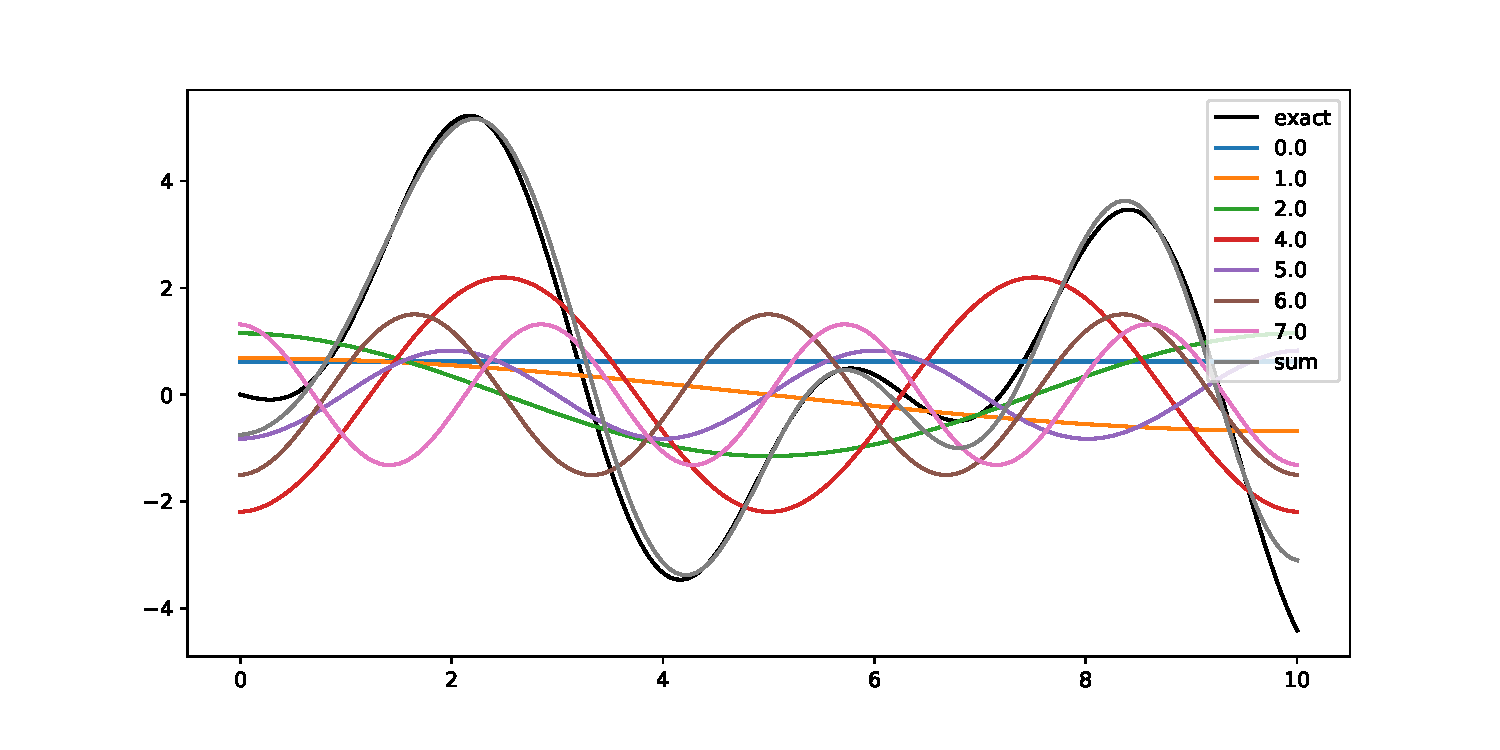
\includegraphics[width=\textwidth]{images/cos1.pdf}
 \caption{The base frequencies}
 \label{fig:cos1}
\end{subfigure}
\quad
\begin{subfigure}{.48\textwidth}
\centering
 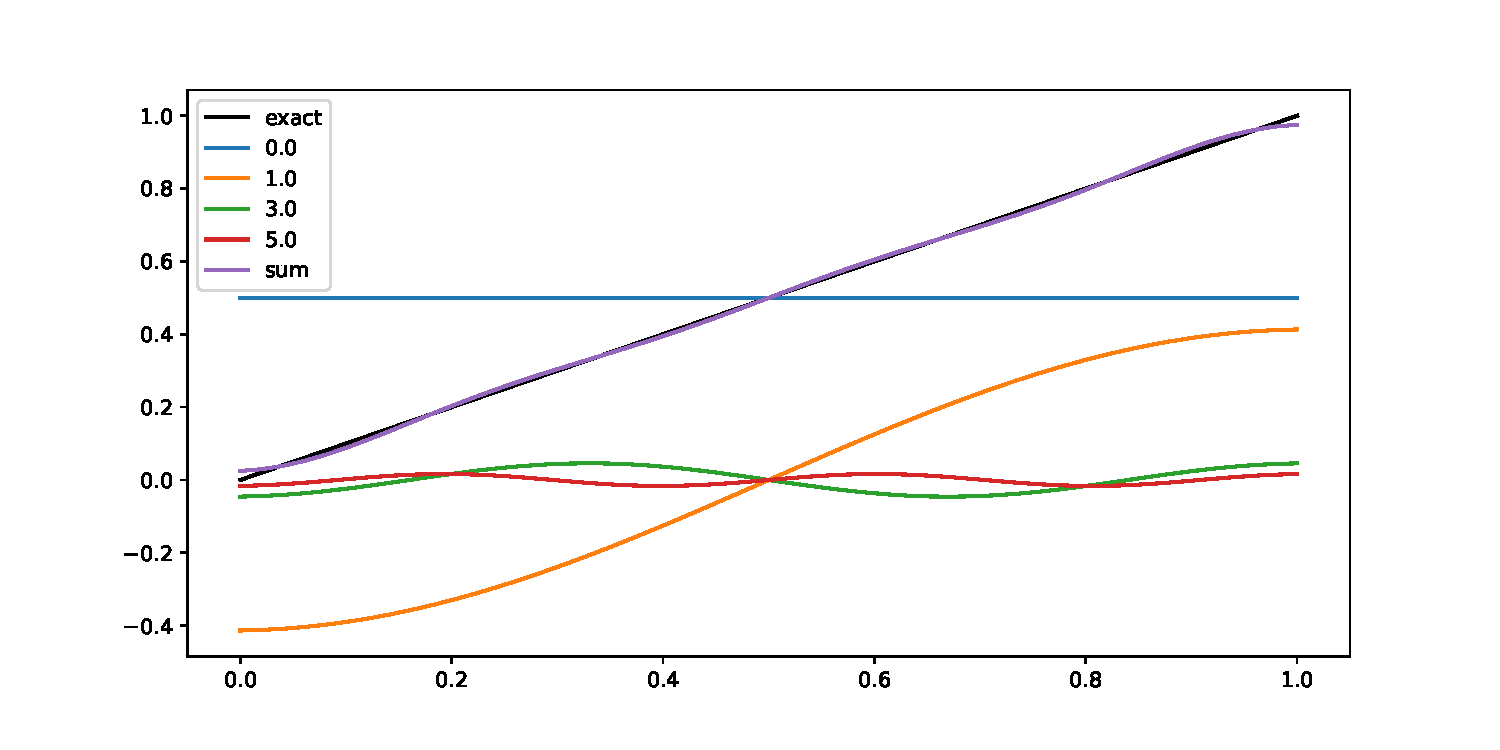
\includegraphics[width=\textwidth]{images/cos2.pdf}
 \caption{The base frequencies}
 \label{fig:cos2}
\end{subfigure}
\caption{The Figures for Problem \ref{prob:base}}
\label{fig:base}
\end{figure}


The two functions depicted in the graphs are $\sin(x/2) + 3\sin(x) - 2\sin(2x)$ and $g(x) = x$.
For $f(x)$ I used 200 data points between 0 and 10 and my cutoff amplitude was 100. For $g(x)$
I used 50 data points between 0 and 1 and my cutoff amplitude was .5.


\end{problem}


\end{document}






































